\documentclass{article}
\usepackage{spconf,amsmath,amssymb,graphicx}
\usepackage{booktabs}
\usepackage{multirow}
\usepackage{xcolor}
\usepackage{cite}
\usepackage{url}

% NOTE: this file targets the official ICASSP two-column "spconf" style
% (spconf.sty + IEEEbib.bst), confirmed against the ICASSP author-kit
% Template.tex. If the conference portal's downloaded kit differs, drop this
% preamble in favor of the official kit and keep only the content below
% \begin{document}.

\title{Longitudinal Drift in sEMG Hand-Gesture Recognition: Robustness Across Decision Paradigms, Architectures, and Individuals}

\name{L.-G. Mac\'ias-Santill\'an, L. I. Barona L\'opez, M. E. Benalc\'azar, \'A. L. Valdivieso Caraguay}
\address{Artificial Intelligence and Computer Vision Research Lab, Departamento de Inform\'atica y\\
Ciencias de la Computaci\'on (DICC), Escuela Polit\'ecnica Nacional, Quito, 170143, Ecuador}

\begin{document}
\maketitle

\begin{abstract}
Surface electromyography (sEMG) is non-stationary, yet most hand-gesture-recognition (HGR) systems are calibrated once and never re-evaluated across sessions. We report a six-month longitudinal study that tests, and separates, three questions usually left unexamined: does a frozen deep representation actually drift; is that drift specific to one architecture family or one decision paradigm; and does the population-average accuracy curve reported in most studies describe any individual user. We freeze a CNN-Transformer-encoder backbone (three capacities) after one calibration session and evaluate two decision heads, a supervised Softmax classifier and a LinUCB contextual bandit, on six later sessions from 19 participants. Two independent two-sample tests (MMD$^2$, domain-classifier $\mathcal{A}$-distance) detect a statistically significant covariate shift in the frozen representation every month ($p<0.05$, Holm-Bonferroni-corrected), while accuracy falls only 4.6--5.9\% across all six backbone-paradigm combinations. Repeating the protocol with two classical, architecturally unrelated baselines (SVM, $k$-NN) reproduces the same qualitative pattern at a larger magnitude, evidence the drop is not an artifact of one architecture. Finally, replacing the pooled population model with 19 independent per-participant models shows that population-averaged stability hides large individual disagreement: between-participant dispersion roughly triples for hand-crafted-feature classifiers after the calibration month, while a Softmax head on the learned representation keeps it flat. These results argue that robustness claims in longitudinal HGR should be checked across architecture family and individual participants, not only across sessions.
\end{abstract}

\begin{keywords}
hand gesture recognition, surface electromyography, covariate shift, contextual bandits, Transformer encoder, longitudinal evaluation
\end{keywords}

\section{Introduction}
\label{sec:intro}

Surface electromyography (sEMG) is a widely used sensing modality for hand-gesture recognition (HGR), with applications in prosthetic control, rehabilitation, and human-machine interaction \cite{Jaramillo2020,Benalcazar2017}. sEMG signals are non-stationary: their statistics change across sessions due to electrode placement, fatigue, and skin impedance \cite{Montazerin2022,transradialSimon}. Despite this, most HGR studies still evaluate a model within a single session or under short-term cross-validation \cite{Jaramillo2020}, and reinforcement-learning-style decision mechanisms remain comparatively unexplored relative to supervised classifiers in this literature \cite{VasconezV2022,VASCONEZ2023}.

This leaves two questions largely untested with a formal procedure, rather than only assumed. First, if a deep feature extractor is frozen after calibration, does its output distribution actually shift over months, independently of whether downstream accuracy changes (a stable accuracy curve can mask a real shift if the decision head happens to compensate for it). Second, once a discriminative representation is learned, does the choice between a supervised decision head and a reinforcement-learning-style one change how the system responds to that shift; contrasting two decision paradigms on an otherwise identical, frozen representation isolates this question in a way that contrasting two architectures cannot, since architecture changes would only speak to representation capacity.

We answer both questions with a longitudinal design, and then stress-test the answer along two axes that longitudinal HGR studies rarely check. A CNN-Transformer-encoder backbone is trained once on session zero (Month~0) and frozen; its 128-d output is tested directly for covariate shift across six later monthly sessions with two independent two-sample tests, and separately scored with a supervised Softmax head and a LinUCB contextual bandit, across three backbone capacities. To test whether any pattern found is specific to this architecture family, we repeat the full protocol with two classical, architecturally unrelated classifiers (SVM, $k$-NN) trained on hand-crafted statistical features. To test whether the population-averaged accuracy curve, the only view most longitudinal HGR studies report, is representative of individual participants, we repeat the protocol once more with 19 independent per-participant models instead of one pooled model.

Our contributions are: (1) statistical evidence, from two independent two-sample tests, that a frozen deep sEMG representation exhibits covariate shift across six months, surviving a Holm-Bonferroni correction for multiple comparisons; (2) a matched comparison of a supervised Softmax head against a LinUCB contextual bandit on the identical frozen representation across three backbone capacities, showing the accuracy drop is governed by backbone capacity, not decision paradigm; (3) evidence, from two classical, architecturally unrelated baselines, that this drop is not confined to the CNN-Transformer-encoder family; and (4) a personalized, per-participant re-analysis showing that population-averaged robustness claims can hide substantial individual disagreement, and that this disagreement is markedly smaller for a learned representation than for hand-crafted features.

\section{Methodology}
\label{sec:method}

\subsection{Longitudinal Protocol and Preprocessing}
Nineteen participants were recorded across seven sessions spanning six months (Month~0 through Month~6). Every model is calibrated once on Month~0 and evaluated, frozen, on Month~1--6; within Month~0, repetitions are split 80/20 between training and validation independently per participant, so all 19 participants appear in every session and only elapsed time varies across evaluations. Eight-channel sEMG is amplitude-normalized, rectified, and low-pass filtered to obtain an envelope, then segmented into 300-sample frames (30-sample stride) labeled by a dual-tolerance overlap rule against the annotated gesture interval. Each frame is converted to a $13\times24\times8$ spectrogram tensor via STFT. Frame-level class imbalance (roughly two-thirds \emph{noGesture}) is corrected with balanced class weights, computed once from Month~0 training and applied identically to the backbone's cross-entropy loss, the Softmax head, and the bandit's reward scale.

\subsection{Transformer-Encoder Backbone and Classical Baselines}
The feature extractor follows an Inception-style convolutional stage \cite{Isabel2023} (six blocks, four parallel branches each) folded into a single Transformer-encoder block ($d_{model}=128$, 8 heads) \cite{Vaswani2017}, trained with cross-entropy on Month~0 and frozen at its final dropout layer, yielding a 128-d representation $\mathbf{z}$ shared by every decision mechanism below. This backbone, at larger scale, previously reached 95.25\% accuracy on a 612-participant sEMG dataset \cite{HGREncoder}, motivating its use here as an architecture with an established track record rather than an untested design. We train the same architecture at three capacities (large: 6 Inception blocks, $d_{model}{=}128$; medium: 4 blocks, $d_{model}{=}64$; small: 2 blocks, $d_{model}{=}32$) to test whether any effect below is an artifact of one network size.

To test whether a drift pattern is specific to this architecture family, we evaluate two classical classifiers sharing no component with it: a support-vector machine \cite{SVM2022} and a $k$-nearest-neighbors classifier \cite{Cipriani2011}, both trained on a hand-crafted 32-d feature vector (mean absolute value, RMS, standard deviation, energy per channel) instead of the learned representation, under the same Month~0-only training rule and class-weight formula. If a drop found only in the Transformer-encoder family later turned out to also appear in these two unrelated classifiers, that would argue the drop reflects the recognition task across sessions rather than one architecture's inductive bias.

\subsection{Covariate-Shift Testing on the Frozen Representation}
We test $\mathbf{z}$ directly for covariate shift between Month~0 and each later month, with two independent two-sample tests, so that a decision head compensating well for a real shift cannot hide it. Maximum Mean Discrepancy (MMD$^2$) is computed with a Gaussian RBF kernel (median-heuristic bandwidth) \cite{Gretton2012MMD}; a domain classifier (5-fold cross-validated logistic regression) predicts Month~0 vs.\ month $m$, converted to the $\mathcal{H}$-divergence-based $\mathcal{A}$-distance $d_{\mathcal{A}}=2(1-2\epsilon)$ \cite{BenDavid2010Domain}. Both statistics use a 2000-iteration permutation test for significance; twelve resulting $p$-values (six months $\times$ two tests) are jointly assessed with a Holm-Bonferroni correction.

\subsection{Decision Mechanisms: Softmax and LinUCB}
A Softmax head ($z$-score-normalized input, weighted cross-entropy, early-stopped on Month~0 validation) instantiates the supervised paradigm. LinUCB \cite{Li2010LinUCB} instantiates a reinforcement-learning paradigm: it treats $\mathbf{z}_t$ as context and each gesture as an arm, selecting $\hat y=\arg\max_i \hat\theta_i^\top \mathbf{x}_t+\alpha\sqrt{\mathbf{x}_t^\top A_i^{-1}\mathbf{x}_t}$, updated via Sherman-Morrison after observing a scalar reward $r_t=\pm w_{c^*}$ (never the true label directly), with sublinear regret guarantees \cite{Chu2011Regret}. Both mechanisms are warm-started once on Month~0 under the same kind of rule, shuffled-epoch training with early stopping on Month~0 validation accuracy, and then frozen (LinUCB drops its exploration term at evaluation time); their epoch budgets differ (Softmax: up to 200 epochs, patience 10; LinUCB: up to 20, patience 5, reflecting its far cheaper per-epoch update) but both are stopped by the same validation criterion rather than a fixed schedule, so any difference between them in Month~1--6 reflects the decision paradigm itself, not one paradigm being cut off early.

\subsection{Personalized Per-Participant Models}
Every model above is a \emph{population} model: one classifier trained on pooled Month~0 data from all 19 participants. A stable population-level curve is consistent both with every participant drifting a little and with a few participants collapsing while the rest stay stable; Section~\ref{sec:results} cannot distinguish these from the population view alone. We therefore repeat the evaluation with one independent classifier per participant, trained and tested using only that participant's own data, for the most stable configuration found per classical family (linear-kernel SVM, $C{=}10$; $k$-NN, $k{=}9$, cosine distance) and for a Softmax head retrained per participant on the frozen small backbone's representation. All 19 participants have complete Month~0--6 data, so none are excluded.

\begin{table}[t]
\caption{Accuracy at Month~0(val) vs.\ Month~6, and the relative drop, for all five models.}
\label{tab:results}
\centering
\resizebox{\linewidth}{!}{%
\begin{tabular}{@{}lcccccc@{}}
\toprule
\multirow{2}{*}{\textbf{Model}} & \multicolumn{3}{c}{\textbf{Softmax}} & \multicolumn{3}{c}{\textbf{LinUCB}} \\
\cmidrule(lr){2-4} \cmidrule(lr){5-7}
 & M0 & M6 & Drop & M0 & M6 & Drop \\
\midrule
Large  & 93.9 & 89.4 & 4.8\% & 93.3 & 87.8 & 5.9\% \\
Medium & 92.0 & 87.8 & 4.6\% & 91.3 & 87.0 & 4.8\% \\
Small  & 86.7 & 82.5 & 4.8\% & 84.6 & 80.7 & 4.6\% \\
\midrule
SVM (Gaussian)     & \multicolumn{3}{c}{73.7 \; 55.4 \; 24.9\%} & \multicolumn{3}{c}{---} \\
$k$-NN ($k{=}1$)   & \multicolumn{3}{c}{92.2 \; 79.2 \; 14.1\%} & \multicolumn{3}{c}{---} \\
\bottomrule
\end{tabular}}
\end{table}

\section{Results}
\label{sec:results}

\subsection{The Frozen Representation Shifts, With a Small Effect Size}
Both MMD$^2$ and the domain-classifier $\mathcal{A}$-distance reject the null hypothesis of no distributional difference at every month ($p<0.05$), and this survives a Holm-Bonferroni correction across all twelve tests, including the largest individual $p$-value (Month~4 MMD, $p=0.034$). The domain classifier's cross-validated accuracy ranges only 52.8--59.4\% against a 50\% chance level ($\mathcal{A}$-distance $\le 0.38$ of 2): the shift is real but small, consistent with Fig.~\ref{fig:covshift}, where MMD$^2$ peaks at Month~5 (0.00467) and dips at Month~4 (0.00048), non-monotonically.

\begin{figure}[t]
\centering

\includegraphics[width=0.85\linewidth]{fig_covariate_shift_en.png}
\caption{MMD$^2$ (left) and domain-classifier $\mathcal{A}$-distance (right) between Month~0 and each later month. Asterisks mark $p<0.05$.}
\label{fig:covshift}
\end{figure}

\subsection{Accuracy Drop is Governed by Architecture Family, Not by Paradigm or Capacity}
Table~\ref{tab:results} reports Month~0(val)-to-Month~6 accuracy for all five models. The three Transformer-encoder backbones drop by a narrow 4.6--5.9\% regardless of capacity or decision paradigm; Fig.~\ref{fig:sl_vs_rl} shows both paradigms tracking each other closely across all seven sessions and three scales (Panel A), while both classical baselines (Panel B) show the same qualitative peak-then-decline shape at a substantially larger magnitude (24.9\% and 14.1\%). Because SVM and $k$-NN share no component with the deep backbone, this argues the pattern reflects the sEMG recognition task across sessions rather than one architecture's inductive bias; because the 4.6--5.9\% band does not widen as backbone capacity shrinks by two orders of magnitude, capacity governs the absolute accuracy level but not how much either paradigm drifts from it.

\begin{figure}[t]
\centering

\includegraphics[width=\linewidth]{fig_sl_vs_rl_scales_en.png}
\caption{Accuracy across seven sessions. Panel A: Softmax vs.\ LinUCB, three backbone capacities. Panel B: SVM and $k$-NN on their own accuracy range.}
\label{fig:sl_vs_rl}
\end{figure}

Every model's single largest step is between Month~0(val) and Month~1, not a gradual month-over-month decline. Two design properties, not a data artifact, explain most of this: Month~0(val) shares its recording session with Month~0(train), while Month~1--6 are each a new session; and every model's stopping point is selected by Month~0(val) accuracy (\texttt{ValidationPatience}), which mechanically favors that split. We could not fully separate this one-time session-identity step from genuine month-over-month drift within the reported drop percentages, and note this as an open question rather than apportion it without direct evidence.

\subsection{Personalized Models: Population Averages Hide Individual Disagreement}
Table~\ref{tab:personal} reports between-participant accuracy dispersion by session for the three personalized configurations of Section~\ref{sec:method}D. For both classical baselines, dispersion roughly triples between Month~0 and Month~1 and stays elevated (11.7--20.5 points across Month~1--6, vs.\ 3.9--6.9 at Month~0); for Softmax on the learned representation of even the smallest backbone, it stays flat (4.1--6.9 points) across all seven sessions (Fig.~\ref{fig:personalsd}). Individually, no participant's trajectory resembles the population-level plateau: some decline sharply and do not recover, others dip and largely recover, and only a minority stay close to Month~0 throughout (the population average is not representative of a typical participant, only of the pooled distribution).

\begin{table}[t]
\caption{Between-participant accuracy SD (points), personalized models.}
\label{tab:personal}
\centering
\resizebox{\linewidth}{!}{%
\begin{tabular}{@{}lccccccc@{}}
\toprule
\textbf{Model} & M0 & M1 & M2 & M3 & M4 & M5 & M6 \\
\midrule
SVM (linear)     & 6.9 & 16.8 & 16.9 & 20.5 & 18.0 & 18.5 & 18.3 \\
$k$-NN ($k{=}9$) & 3.9 & 12.4 & 14.5 & 16.2 & 11.9 & 15.8 & 11.7 \\
Softmax (small)  & 5.6 & 4.6  & 5.4  & 4.1  & 5.4  & 6.9  & 6.8  \\
\bottomrule
\end{tabular}}
\end{table}

\begin{figure}[t]
\centering
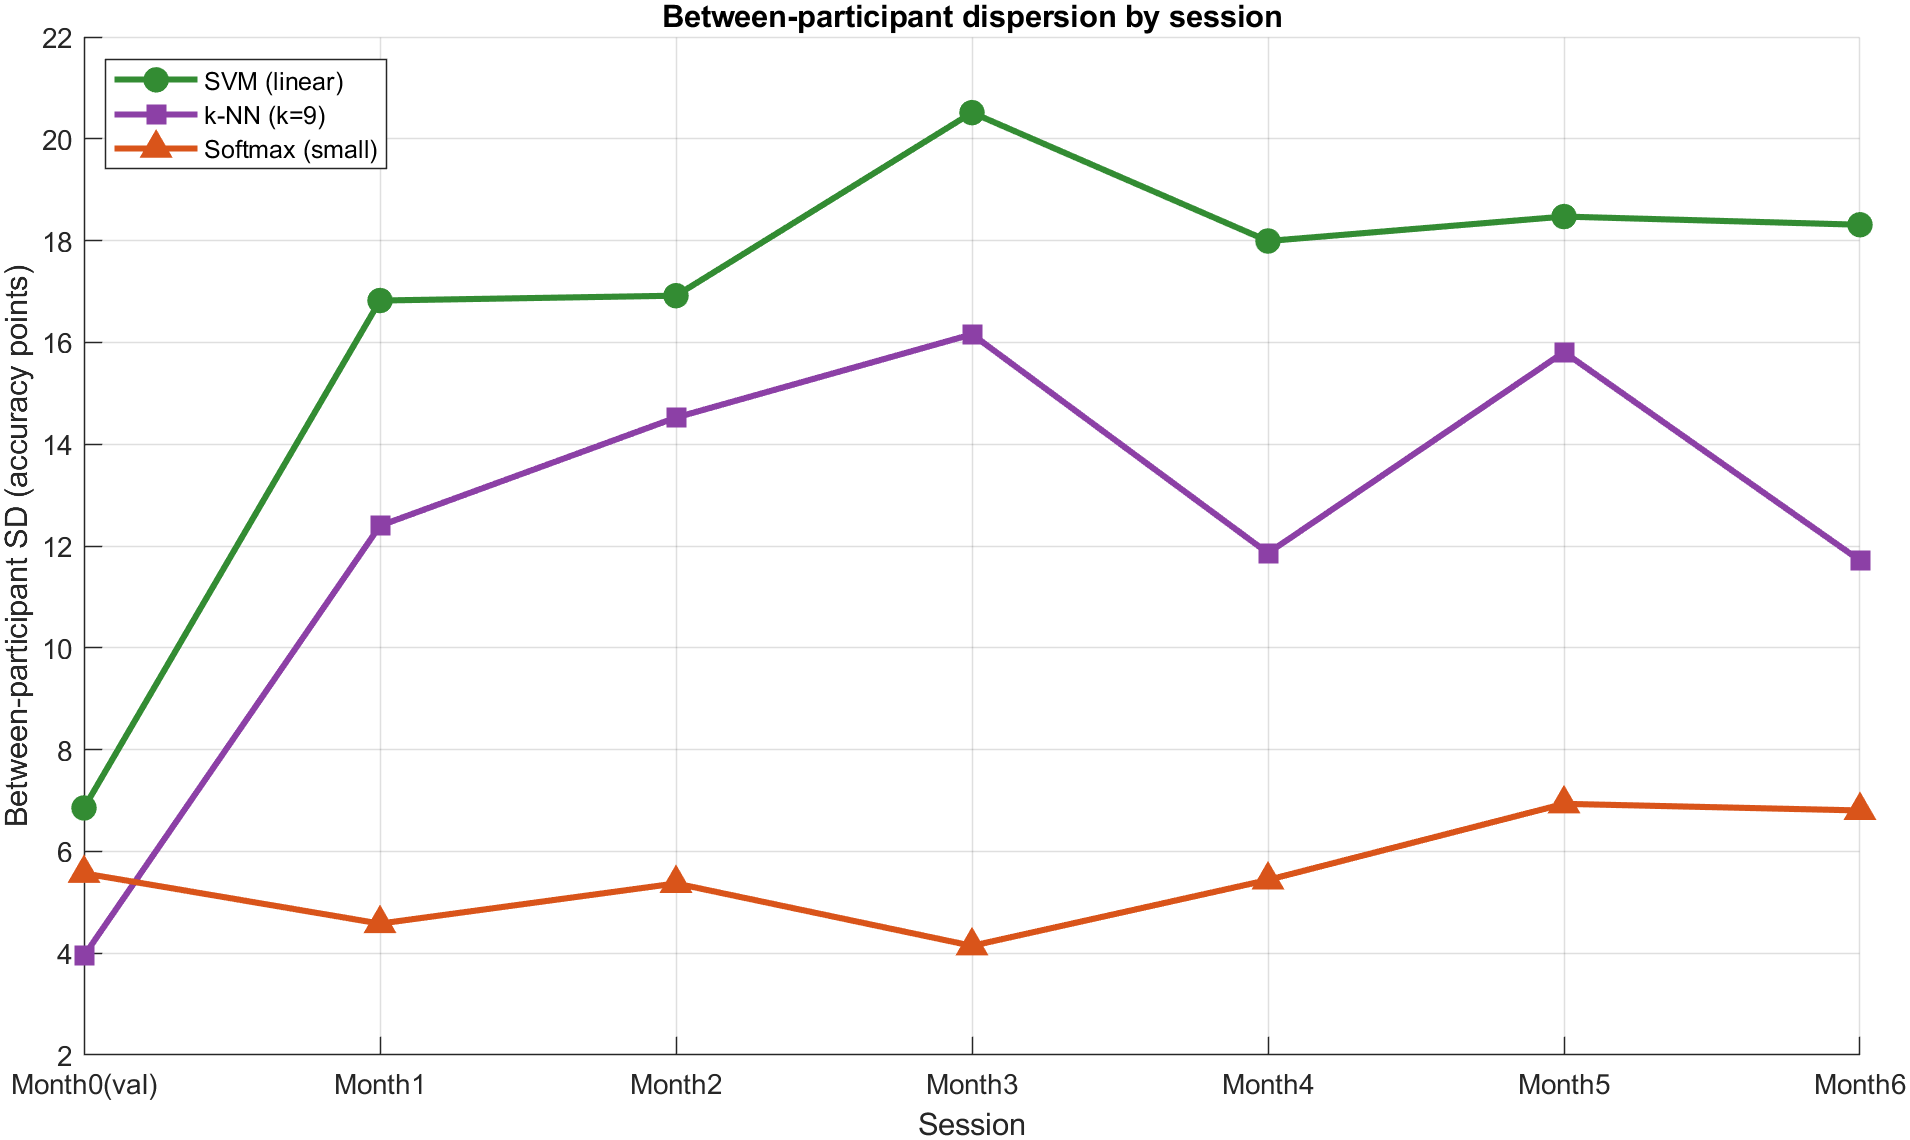
\includegraphics[width=0.9\linewidth]{fig_personalizado_sd_por_mes_en.png}
\caption{Between-participant accuracy SD by session, personalized models. Classical baselines' dispersion jumps at Month~1 and stays elevated; the learned-representation dispersion stays flat.}
\label{fig:personalsd}
\end{figure}

\section{Discussion}
\label{sec:discussion}

Together, these results support a narrower claim than either ``there is no drift'' or ``the decision paradigm determines robustness.'' A frozen sEMG representation shifts measurably but modestly across six months; the resulting accuracy decline is governed by backbone capacity and, more broadly, by whether the model uses a learned or hand-crafted representation at all, not by whether its decision head is a supervised classifier or a bandit. This decline is not confined to one architecture family, and the population-level view used to reach it is not representative of individual participants: two classical, architecturally unrelated classifiers reproduce the pattern at a larger magnitude, and personalized models reveal that hand-crafted features leave individuals far more unevenly exposed to drift than a learned representation does, even at minimal backbone capacity.

This study has four limitations. First, LinUCB is evaluated frozen and purely exploitative after warm-start; a permanently online, classifier-guided variant \cite{LinPaskettYang2025} was set aside to keep both paradigms under matched, non-adaptive conditions. Second, neither MMD$^2$ nor the accuracy drop is monotonic across months, and we lack a mechanistic explanation. Third, the backbone is trained once with cross-entropy and frozen; LinUCB never shapes the representation itself, so this is not a test of end-to-end reinforcement learning. Fourth, personalized results use only the smallest backbone for computational cost, so we do not yet know whether the flat between-participant dispersion found here holds at larger capacity.

\section{Conclusion}
\label{sec:conclusion}

A frozen sEMG representation exhibits a small but statistically real covariate shift over six months, corresponding to a modest 4.6--5.9\% accuracy decline that is consistent across three Transformer-encoder capacities and both a supervised Softmax head and a LinUCB bandit (decision paradigm does not change how much the system drifts). This decline generalizes beyond the Transformer-encoder family to two classical, architecturally unrelated classifiers, and the population-averaged curves used to establish it do not represent individual participants: personalized models show individual dispersion that is roughly three times smaller for a learned representation than for hand-crafted features. Future work should test whether this holds at a larger cohort and larger personalized-model capacity, and with the backbone trained end-to-end from reward alone rather than frozen after supervised pretraining.

\section*{Data and Code Availability}
The longitudinal sEMG dataset used in this study is not publicly released: participant consent does not yet extend to unrestricted public redistribution (broadening it is in progress), and the dataset remains under active use by other ongoing studies in the same laboratory. It is available from the authors upon reasonable request. The complete analysis code is publicly available at \url{https://github.com/laboratorioAI/hgr-emg-longitudinal-study}.

\section*{Compliance with Ethical Standards}
All participants provided written informed consent prior to data collection, in accordance with the protocols of the Artificial Intelligence and Computer Vision Research Lab, Escuela Polit\'ecnica Nacional.

\section*{Acknowledgment}
The authors thank the Artificial Intelligence and Computer Vision Research Lab, Escuela Polit\'ecnica Nacional, for the data collection infrastructure used in this study.

\bibliographystyle{IEEEbib}
\bibliography{bib}

\end{document}
